\section{The Dot Product}\label{sec:dot_product}

The previous section introduced vectors and described how to add them together and how to multiply them by scalars. This section introduces \emph{a} multiplication on vectors called the \textbf{dot product}.

\definition{def:dot_product}{Dot Product}
{\begin{enumerate}
	\item Let $\vec u = \la u_1,u_2\ra$ and $\vec v = \la v_1,v_2\ra$  in $\mathbb{R}^2$. The \textbf{dot product} of $\vec u$ and $\vec v$, denoted \dotp uv, is 
	\index{dot product!definition}\index{vectors!dot product}
	$$\dotp uv = u_1v_1+u_2v_2.$$
	\item Let $\vec u = \la u_1,u_2,u_3\ra$ and $\vec v = \la v_1,v_2,v_3\ra$  in $\mathbb{R}^3$. The \textbf{dot product} of $\vec u$ and $\vec v$, denoted \dotp uv, is 
	$$\dotp uv = u_1v_1+u_2v_2+u_3v_3.$$
\end{enumerate}
}

Note how this product of vectors returns a \emph{scalar}, not another vector. We practice evaluating a dot product in the following example, then we will discuss why this product is useful.\\

\example{ex_dotp1}{Evaluating dot products}{
\begin{enumerate}
	\item Let $\vec u=\la 1,2\ra$, $\vec v=\la 3,-1\ra$ in $\mathbb{R}^2$. Find \dotp uv.
	\item Let $\vec x = \la 2,-2,5\ra $ and $\vec y = \la -1, 0, 3\ra$ in $\mathbb{R}^3$. Find \dotp xy.
\end{enumerate} 
}
{\begin{enumerate}
	\item Using Definition \ref{def:dot_product}, we have $$\dotp uv = 1(3)+2(-1) = 1.$$
	\item	Using the definition, we have
	$$\dotp xy = 2(-1)  -2(0) + 5(3) = 13.$$
\end{enumerate}
\vskip-\baselineskip
}\\

The dot product, as shown by the preceding example, is very simple to evaluate. It is only the sum of products. While the definition gives no hint as to why we would care about this operation, there is an amazing connection between the dot product and angles formed by the vectors. Before stating this connection, we give a theorem stating some of the properties of the dot product.

\theorem{thm:dot_product_properties}{Properties of the Dot Product}
{Let $\vec u$, $\vec v$ and $\vec w$ be vectors in $\mathbb{R}^2$ or $\mathbb{R}^3$ and let $c$ be a scalar.\index{dot product!properties}\index{vectors!dot product}
\begin{enumerate}
	\item \parbox{150pt}{$\dotp uv = \dotp vu$}{Commutative Property}
	\item \parbox{150pt}{$\vec u\cdot(\vec v+\vec w) = \dotp uv + \dotp uw$}{Distributive Property}
	\item	$c(\dotp uv) = (c\vec u)\cdot \vec v = \vec u \cdot (c\vec v)$
	\item	$\dotp 0v = 0$
	\item	$\dotp vv=\norm{\vec v}^2 $
\end{enumerate}
}

The last statement of the theorem makes a handy connection between the magnitude of a vector and the dot product with itself. 
Our definition and theorem give properties of the dot product, but we are still likely wondering ``What does the dot product \emph{mean}?'' It is helpful to understand that the dot product of a vector with itself is connected to its magnitude.

The next theorem extends this understanding by connecting the dot product to magnitudes and angles. Given vectors $\vec u$ and $\vec v$ in the plane, an angle $\theta$ is clearly formed when $\vec u$ and $\vec v$ are drawn with the same initial point as illustrated in Figure \ref{fig:dotpangle}(a). (We always take $\theta$ to be the angle in $[0,\pi]$ as two angles are actually created.) 
\mtable{.5}{Illustrating the angle formed by two vectors with the same initial point.}{fig:dotpangle}{%
\begin{tabular}{c}
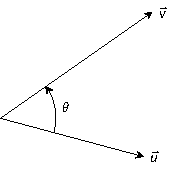
\includegraphics{figures/figdotpangle}\\
(a)\\[15pt]
\myincludegraphicsthree{width=125pt,3Dmenu,activate=onclick,deactivate=onclick,
3Droll=0,
3Dortho=0.0045,
3Dc2c=.54 .61 .58,
3Dcoo=0 0 40,
3Droo=170,
3Dlights=Headlamp,add3Djscript=asylabels.js}{}{figures/figdotpangle3D}\\
%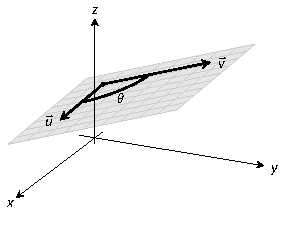
\includegraphics{figures/figdotpangle3D}\\
(b)
\end{tabular}
}

The same is also true of 2 vectors in space: given $\vec u$ and $\vec v$ in $\mathbb{R}^3$ with the same initial point, there is a plane that contains both $\vec u$ and $\vec v$. (When $\vec u$ and $\vec v$ are co-linear, there are infinite planes that contain both vectors.) In that plane, we can again find an angle $\theta$ between them (and again, $0\leq \theta\leq \pi$). This is illustrated in Figure \ref{fig:dotpangle}(b).

The following theorem connects this angle $\theta$ to the dot product of $\vec u$ and $\vec v$.

\theorem{thm:dot_product}{The Dot Product and Angles}
{Let $\vec u$ and $\vec v$ be vectors in $\mathbb{R}^2$ or $\mathbb{R}^3$. Then 
$$\dotp uv = \norm{\vec u}\,\norm{\vec v} \cos\theta,$$
where $\theta$, $0\leq\theta\leq \pi$, is the angle between $\vec u$ and $\vec v$.
\index{dot product!properties}\index{vectors!dot product}
}

Using Theorem \ref{thm:dot_product_properties}, we can rewrite this theorem as
$$\frac{\vec u}{\norm{\vec u}}\cdot \frac{\vec v}{\norm{\vec v}} = \cos \theta.$$
Note how on the left hand side of the equation, we are computing the dot product of two unit vectors. Recalling that unit vectors essentially only provide direction information, we can informally restate Theorem \ref{thm:dot_product} as saying ``The dot product of two directions gives the cosine of the angle between them.''


When $\theta$ is an acute angle (i.e., $0\leq \theta <\pi/2$), $\cos \theta$ is positive; when $\theta = \pi/2$, $\cos \theta = 0$; when $\theta$ is an obtuse angle ($\pi/2<\theta \leq \pi$), $\cos \theta$ is negative. Thus the sign of the dot product gives a general indication of the angle between the vectors, illustrated in Figure \ref{fig:dotpsign}.

\begin{center}
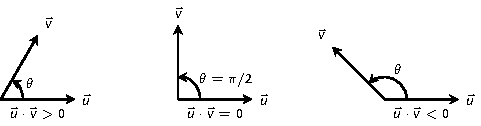
\includegraphics{figures/figdotpanglesign}
\captionsetup{type=figure}
\caption{Illustrating the relationship between the angle between vectors and the sign of their dot product.}
\label{fig:dotpsign}
\end{center}
\vskip\baselineskip

We \emph{can} use Theorem \ref{thm:dot_product} to compute the dot product, but generally this theorem is used to find the angle between known vectors (since the dot product is generally easy to compute). To this end, we rewrite the theorem's equation as
$$\cos \theta = \frac{\dotp uv}{\norm{\vec u}\norm{\vec v}} \quad \Leftrightarrow \quad \theta = \cos^{-1}\left(\frac{\dotp uv}{\norm{\vec u}\norm{\vec v}}\right).$$

We practice using this theorem in the following example.\\

\mfigure{.3}{Vectors used in Example \ref{ex_dotp2}.}{fig:dotp2}{figures/figdotp2}
\example{ex_dotp2}{Using the dot product to find angles}{
Let $\vec u = \la 3,1\ra$, $\vec v = \la -2,6\ra$ and $\vec w = \la -4,3\ra$, as shown in Figure \ref{fig:dotp2}. Find the angles $\alpha$, $\beta$ and $\theta$.
}
{We start by computing the magnitude of each vector.
$$\norm{\vec u} = \sqrt{10};\quad \norm{\vec v} = 2\sqrt{10};\quad \norm{\vec w} = 5.$$
We now apply Theorem \ref{thm:dot_product} to find the angles.
\begin{align*}
\alpha &= \cos^{-1}\left(\frac{\dotp uv}{(\sqrt{10})(2\sqrt{10})}\right) \\
			&= \cos^{-1}(0) = \frac{\pi}2 = 90^\circ.
\end{align*}
\begin{align*}
\beta &= \cos^{-1}\left(\frac{\dotp vw}{(2\sqrt{10})(5)}\right) \\
			&= \cos^{-1}\left(\frac{26}{10\sqrt{10}}\right) \\
					&\approx 0.6055 \approx 34.7^\circ.\\[10pt]
\theta &= \cos^{-1}\left(\frac{\dotp uw}{(\sqrt{10})(5)}\right) \\
				&= \cos^{-1}\left(\frac{-9}{5\sqrt{10}}\right) \\
				&\approx 2.1763 \approx 124.7^\circ
\end{align*}
\vskip-\baselineskip
}\\

We see from our computation that $\alpha + \beta = \theta$, as indicated by Figure \ref{fig:dotp2}. While we knew this should be the case, it is nice to see that this non-intuitive formula indeed returns the results we expected.

We do a similar example next in the context of vectors in space.\\

\mfigurethree{width=150pt,3Dmenu,activate=onclick,deactivate=onclick,
3Droll=0,
3Dortho=0.0045,
3Dc2c=.89 .4 .23,
3Dcoo=10 50 46,
3Droo=200,
3Dlights=Headlamp,add3Djscript=asylabels.js}{}{.4}{Vectors used in Example \ref{ex_dotp3}.}{fig:dotp3}{figures/figdotp3}%
%\mfigure{.4}{Vectors used in Example \ref{ex_dotp3}.}{fig:dotp3}{figures/figdotp3}
\example{ex_dotp3}{Using the dot product to find angles}{
Let $\vec u = \la 1,1,1\ra$, $\vec v = \la -1,3,-2\ra$ and $\vec w = \la -5,1,4\ra$, as illustrated in Figure \ref{fig:dotp3}. Find the angle between each pair of vectors.}
{\begin{enumerate}
	\item Between $\vec u$ and $\vec v$:
	\begin{align*}
	\theta &= \cos^{-1}\left(\frac{\dotp uv}{\norm{\vec u}\norm{\vec v}}\right)\\
					&= \cos^{-1}\left(\frac{0}{\sqrt{3}\sqrt{14}}\right)\\
					&= \frac{\pi}2.
	\end{align*}
	\item	Between $\vec u$ and $\vec w$:
	\begin{align*}
	\theta &= \cos^{-1}\left(\frac{\dotp uw}{\norm{\vec u}\norm{\vec w}}\right)\\
					&= \cos^{-1}\left(\frac{0}{\sqrt{3}\sqrt{42}}\right)\\
					&= \frac{\pi}2.
	\end{align*}
	\item	Between $\vec v$ and $\vec w$:
	\begin{align*}
	\theta &= \cos^{-1}\left(\frac{\dotp vw}{\norm{\vec v}\norm{\vec w}}\right)\\
					&= \cos^{-1}\left(\frac{0}{\sqrt{14}\sqrt{42}}\right)\\
					&= \frac{\pi}2.
	\end{align*}
\end{enumerate}
While our work shows that each angle is $\pi/2$, i.e.,  $90^\circ$, none of these angles looks to be a right angle in Figure \ref{fig:dotp3}. Such is the case when drawing three--dimensional objects on the page.
}\\

All three angles between these vectors was $\pi/2$, or $90^\circ$. We know from geometry and everyday life that $90^\circ$ angles are ``nice'' for a variety of reasons, so it should seem significant that these angles are all $\pi/2$. Notice the common feature in each calculation (and also the calculation of $\alpha$ in Example \ref{ex_dotp2}): the dot products of each pair of angles was 0. We use this as a basis for a definition of the term \textbf{orthogonal}, which is essentially synonymous to \textit{perpendicular}.

\definition{def:orthogonal}{Orthogonal}
{Vectors $\vec u$ and $\vec v$ are \textbf{orthogonal} if their dot product is 0.
\index{orthogonal}\index{perpendicular|see{orthogonal}}\index{vectors!orthogonal}
}

\mnote{.4}{\textbf{Note:} The term \textit{perpendicular} originally referred to lines. As mathematics progressed, the concept of ``being at right angles to'' was applied to other objects, such as vectors and planes, and the term \emph{orthogonal} was introduced. It is especially used when discussing objects that are hard, or impossible, to visualize: two vectors in 5-dimensional space are orthogonal if their dot product is 0. It is not wrong to say they are \textit{perpendicular}, but common convention gives preference to the word \textit{orthogonal}.
}

\example{ex_dotp8}{Finding orthogonal vectors}{
Let $\vec u = \la 3,5\ra$ and $\vec v = \la 1,2,3\ra$. 
\begin{enumerate}
	\item Find two vectors in $\mathbb{R}^2$ that are orthogonal to $\vec u$.
	\item	Find two non--parallel vectors in $\mathbb{R}^3$ that are orthogonal to $\vec v$.
\end{enumerate}
}
{\begin{enumerate}
	\item Recall that a line perpendicular to a line with slope $m$ has slope $-1/m$, the ``opposite reciprocal slope.'' We can think of the slope of $\vec u$ as $5/3$, its ``rise over run.'' A vector orthogonal to $\vec u$ will have slope $-3/5$. There are many such choices, though all parallel:
	$$\la -5,3\ra \quad \text{or} \quad\la 5,-3\ra \quad \text{or} \quad \la -10,6\ra\quad \text{or} \quad \la 15,-9\ra,\text{etc.}$$
	\item		There are infinite directions in space orthogonal to any given direction, so there are an infinite number of non--parallel vectors orthogonal to $\vec v$. Since there are so many, we have great leeway in finding some.
	
	One way is to arbitrarily pick values for the first two components, leaving the third unknown. For instance, let $\vec v_1 = \la 2,7,z\ra$. If $\vec v_1$ is to be orthogonal to $\vec v$, then $\vec v_1\cdot\vec v = 0$, so 
	$$2+14+3z=0 \quad \Rightarrow z = \frac{-16}{3}.$$
	So $\vec v_1 = \la 2, 7, -16/3\ra$ is orthogonal to $\vec v$. We can apply a similar technique by leaving the first or second component unknown.
	
	Another method of finding a vector orthogonal to $\vec v$ mirrors what we did in part 1. Let $\vec v_2 = \la-2,1,0\ra$. Here we switched the first two components of $\vec v$, changing the sign of one of them (similar to the ``opposite reciprocal'' concept before). Letting the third component be 0 effectively ignores the third component of $\vec v$, and it is easy to see that 
	$$\vec v_2\cdot\vec v = \la -2,1,0\ra\cdot\la 1,2,3\ra = 0.$$
	Clearly $\vec v_1$ and $\vec v_2$ are not parallel.
\end{enumerate}
\vskip-1.5\baselineskip
}\\

An important construction is illustrated in Figure \ref{fig:dotpproj}, where vectors $\vec u$ and $\vec v$ are sketched. In part (a), a dotted line is drawn from the tip of $\vec u$ to the line containing $\vec v$, where the dotted line is orthogonal to $\vec v$. In part (b), the dotted line is replaced with the vector $\vec z$ and  $\vec w$ is formed, parallel to $\vec v$. It is clear by the diagram that $\vec u = \vec w+\vec z$. What is important about this construction is this: $\vec u$ is \emph{decomposed} as the sum of two vectors, one of which is parallel to $\vec v$ and one that is perpendicular to $\vec v$. It is hard to overstate the importance of this construction (as we'll see in upcoming examples). 

The vectors $\vec w$, $\vec z$ and $\vec u$ as shown in Figure \ref{fig:dotpproj} (b) form a right triangle, where the angle between $\vec v$ and $\vec u$ is labeled $\theta$. We can find $\vec w$ in terms of $\vec v$ and $\vec u$.

Using trigonometry, we can state that 
\begin{equation}
\norm{\vec w} = \norm{\vec u}\cos \theta. \label{eq:proj1}
\end{equation}
\mtable{.450}{Developing the construction of the \emph{orthogonal projection}.}{fig:dotpproj}{%
\begin{tabular}{c}
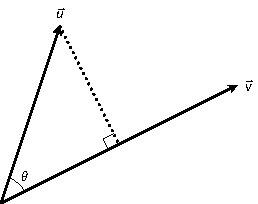
\includegraphics{figures/figdotpproja}\\
(a)\\[15pt]
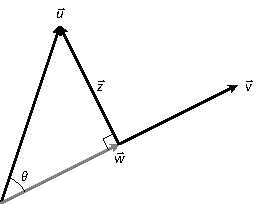
\includegraphics{figures/figdotpprojb}\\
(b)
\end{tabular}
}

We also know that $\vec w$ is parallel to to $\vec v$\,; that is, the direction of $\vec w$ is the direction of $\vec v$, described by the unit vector $\vec v/\norm{\vec v}$. The vector $\vec w$ is the vector in the direction $\vec v/\norm{\vec v}$ with magnitude $\norm{\vec u}\cos \theta$:
\begin{align*}
\vec w &= \Big(\norm{\vec u}\cos\theta \Big)\frac{1}{\norm{\vec v}}\vec v.
\intertext{Replace $\cos\theta$ using Theorem \ref{thm:dot_product}:}
			&= \left(\norm{\vec u}\frac{\dotp uv}{\norm{\vec u}\norm{\vec v}}\right)\frac{1}{\norm{\vec v}} \vec v\\ 
			&= \frac{\dotp uv}{\norm{\vec v}^2}\vec v.
			\intertext{Now apply Theorem \ref{thm:dot_product_properties}.}
			&= \frac{\dotp uv}{\dotp vv}\vec v.
\end{align*}

Since this construction is so important, it is given a special name.

\definition{def:orthogonal_projection}{Orthogonal Projection}
{Let $\vec u$ and $\vec v\neq \vec0$ be given. The \textbf{orthogonal projection of $\vec u$ onto $\vec v$}, denoted $\proj uv$, is 
\index{orthogonal projection}\index{vectors!orthogonal projection}
$$\proj uv = \frac{\dotp uv}{\dotp vv}\vec v.$$
}

\example{ex_dotp4}{Computing the orthogonal projection}{
\begin{enumerate}
	\item Let $\vec u= \la -2,1\ra$ and $\vec v=\la 3,1\ra$. Find $\proj uv$, and sketch all three vectors with initial points at the origin.
	\item	Let $\vec w = \la 2,1,3\ra$ and $\vec x = \la 1,1,1\ra$. Find $\proj wx$, and sketch all three vectors with initial points at the origin.
\end{enumerate}
}
{\begin{enumerate}
	\item Applying Definition \ref{def:orthogonal_projection}, we have
	\begin{align*}
	\proj uv &= \frac{\dotp uv}{\dotp vv}\vec v \\
					&= \frac{-5}{10}\la 3,1\ra\\
					&= \la -\frac32,-\frac12\ra.
	\end{align*}
	Vectors $\vec u$, $\vec v$ and $\proj uv$ are sketched in Figure \ref{fig:dotp4}(a). Note how the projection is parallel to $\vec v$; that is, it lies on the same line through the origin as $\vec v$, although it points in the opposite direction. That is because the angle between $\vec u$ and $\vec v$ is obtuse (i.e., greater than $90^\circ$).
\mtable{.63}{Graphing the vectors used in Example \ref{ex_dotp4}.}{fig:dotp4}{%
\begin{tabular}{c}
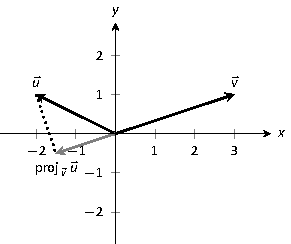
\includegraphics{figures/figdotp4a}\\
(a)\\[15pt]
\myincludegraphicsthree{width=100pt,3Dmenu,activate=onclick,deactivate=onclick,
3Droll=0,
3Dortho=0.0046,
3Dc2c=.9 .12 .42,
3Dcoo=0 50 30,
3Droo=250,
3Dlights=Headlamp,add3Djscript=asylabels.js}{}{figures/figdotp4b}\\
%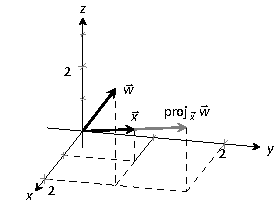
\includegraphics{figures/figdotp4b}\\
(b)\\[15pt]
\myincludegraphicsthree{width=100pt,3Dmenu,activate=onclick,deactivate=onclick,
3Droll=0,
3Dortho=0.0046,
3Dc2c=.29 .77 .56,
3Dcoo=50 0 40,
3Droo=250,
3Dlights=Headlamp,add3Djscript=asylabels.js}{}{figures/figdotp4c}\\
%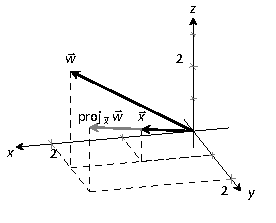
\includegraphics{figures/figdotp4c}\\
(c)\\[15pt]
\end{tabular}
}	
	
	\item		Apply the definition:
	\begin{align*}
	\proj wx &= \frac{\dotp wx}{\dotp xx}\vec x \\
					&= \frac{6}{3}\la 1,1,1\ra\\
					&= \la 2,2,2\ra.
	\end{align*}
	These vectors are sketched in Figure \ref{fig:dotp4}(b), and again in part (c) from a different perspective. Because of the nature of graphing these vectors, the sketch in part (b) makes it difficult  to recognize that the drawn projection has the geometric properties it should. The graph shown in part (c) illustrates these properties better.
\end{enumerate}
\vskip-\baselineskip
}\\

A special case of orthogonal projection occurs when $\vec v$ is a unit vector. In this situation, the formula for the orthogonal projection of a vector $\vec u$ onto $\vec v$ reduces to just $\proj uv = (\vec u\cdot\vec v)\vec v$, as $\vec v\cdot\vec v = 1$.

This gives us a new understanding of the dot product. When $\vec v$ is a unit vector, essentially providing only direction information, the dot product of $\vec u$ and $\vec v$ gives ``how much of $\vec u$ is in the direction of $\vec v$.'' This use of the dot product will be very useful in future sections.\\

\mfigure{.23}{Illustrating the orthogonal projection.}{fig:dotpprojc}{figures/figdotpprojc}
Now consider Figure \ref{fig:dotpprojc} where the concept of the orthogonal projection is again illustrated. It is clear that 
\begin{equation}
\vec u = \proj uv + \vec z.
\label{eq:orthogproj}
\end{equation} As we know what $\vec u$ and $\proj uv$ are, we can solve for $\vec z$ and state that
$$\vec z = \vec u - \proj uv.$$
This leads us to rewrite Equation \eqref{eq:orthogproj} in a seemingly silly way: $$\vec u = \proj uv + (\vec u - \proj uv).$$
This is not nonsense, as pointed out in the following Key Idea. (Notation note: the expression ``$\parallel \vec y$\,'' means ``is parallel to $\vec y$.'' We can use this notation to state ``$\vec x\parallel\vec y$\,'' which means ``$\vec x$ is parallel to $\vec y$.'' The expression ``$\perp \vec y$\,'' means ``is orthogonal to $\vec y$,'' and is used similarly.)

\keyidea{idea:orthog_proj}{Orthogonal Decomposition of Vectors}
{Let $\vec u$ and $\vec v$ be given. Then $\vec u$ can be written as the sum of two vectors, one of which is parallel to $\vec v$, and one of which is orthogonal to $\vec v$:
\index{orthogonal decomposition of vectors}\index{orthogonal!decomposition}\index{vectors!orthogonal decomposition}
$$\vec u = \underbrace{\proj uv}_{\parallel\ \vec v}\ +\  (\underbrace{\vec u-\proj uv}_{\perp\ \vec v}).$$
}

We illustrate the use of this equality in the following example.\\

\example{ex_dotp5}{Orthogonal decomposition of vectors}{
\begin{enumerate}
	\item Let $\vec u = \la -2,1\ra $ and $\vec v = \la 3,1\ra$ as in Example \ref{ex_dotp4}. Decompose $\vec u$ as the sum of a vector parallel to $\vec v$ and a vector orthogonal to $\vec v$.
	\item	Let $\vec w =\la 2,1,3\ra$ and $\vec x  =\la 1,1,1\ra$ as in Example \ref{ex_dotp4}. Decompose $\vec w$ as the sum of a vector parallel to $\vec x$ and a vector orthogonal to $\vec x$.
\end{enumerate}
}
{\begin{enumerate}
	\item In Example \ref{ex_dotp4}, we found that $\proj uv = \la -1.5,-0.5\ra$. Let $$\vec z = \vec u - \proj uv = \la -2,1\ra - \la -1.5,-0.5\ra = \la-0.5, 1.5\ra.$$
	Is $\vec z$ orthogonal to $\vec v$\,? (I.e, is $\vec z \perp\vec v$\ ?) We check for orthogonality with the dot product:
	$$\dotp zv = \la -0.5,1.5\ra \cdot \la 3,1\ra =0.$$
	Since the dot product is 0, we know $\vec z \perp \vec v$. Thus:
	\begin{align*}
	\vec u &= \proj uv\ +\ (\vec u - \proj uv) \\
	\la -2,1\ra &= \underbrace{\la -1.5,-0.5\ra}_{\parallel\ \vec v}\ +\ \underbrace{\la -0.5,1.5\ra}_{\perp \ \vec v}.
	\end{align*}
	
	\item	We found in Example \ref{ex_dotp4} that $\proj wx = \la 2,2,2\ra$. Applying the Key Idea, we have:
	$$\vec z = \vec w - \proj wx = \la 2,1,3\ra  - \la 2,2,2\ra = \la 0,-1,1\ra.$$ We check to see if $\vec z \perp \vec x$:
	$$\dotp zx = \la 0,-1,1\ra \cdot \la 1,1,1\ra = 0.$$
	Since the dot product is 0, we know the two vectors are orthogonal.
	We now write $\vec w$ as the sum of two vectors, one parallel and one orthogonal to $\vec x$:
	\begin{align*}
	\vec w &= \proj wx\ +\ (\vec w - \proj wx) \\
	\la 2,1,3\ra &= \underbrace{\la 2,2,2\ra}_{\parallel\ \vec x}\ +\ \underbrace{\la 0,-1,1\ra}_{\perp \ \vec x} 
	\end{align*}
\end{enumerate}
\vskip-\baselineskip
}\\

We give an example of where this decomposition is useful.\\

\example{ex_dotp6}{Orthogonally decomposing a force vector}{
Consider Figure \ref{fig:dotp6}(a), showing a box weighing 50lb on a ramp that rises 5ft over a span of 20ft. Find the components of force, and their magnitudes, acting on the box (as sketched in part (b) of the figure):
\mtable{.4}{Sketching the ramp and box in Example \ref{ex_dotp6}. Note: \textit{The vectors are not drawn to scale.}}{fig:dotp6}{%
\begin{tabular}{c}
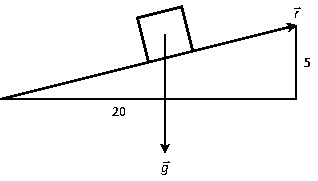
\includegraphics{figures/figdotp6}\\
(a)\\[15pt]
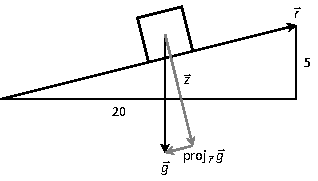
\includegraphics{figures/figdotp6b}\\
(b)
\end{tabular}
}
\begin{enumerate}
	\item in the direction of the ramp, and
	\item	orthogonal to the ramp.
\end{enumerate}
}
{As the ramp rises 5ft over a horizontal distance of 20ft, we can represent the direction of the ramp with the vector $\vec r= \la 20,5\ra$. Gravity pulls down with a force of 50lb, which we represent with $\vec g = \la 0,-50\ra$. 
\begin{enumerate}
	\item To find the force of gravity in the direction of the ramp, we compute $\proj gr$:
	\begin{align*}
	\proj gr &= \frac{\dotp gr}{\dotp rr}\vec r\\
					&=  \frac{-250}{425}\la 20,5\ra\\
					&= \la -\frac{200}{17},-\frac{50}{17}\ra \approx \la -11.76,-2.94\ra.
	\end{align*}
	The magnitude of $\proj gr$ is $\norm{\proj gr} = 50/\sqrt{17} \approx 12.13\text{lb}$. Though the box weighs 50lb, a force of about 12lb is enough to keep the box from sliding down the ramp.
	
	\item		To find the component $\vec z$ of gravity orthogonal to the ramp, we use Key Idea \ref{idea:orthog_proj}.
	\begin{align*}
	\vec z &= \vec g - \proj gr \\
					&= \la \frac{200}{17},-\frac{800}{17}\ra \approx \la 11.76,-47.06\ra.
	\end{align*}
	The magnitude of this force is $\norm{\vec z} \approx 48.51$lb. In physics and engineering, knowing this force is important when computing things like static frictional force. (For instance, we could easily compute if the static frictional force alone was enough to keep the box from sliding down the ramp.)
\end{enumerate}
\vskip-\baselineskip
}\\

\noindent\textbf{\large Application to Work}\\

In physics, the application of a force $F$ to move an object in a straight line a distance $d$ produces \emph{work}; the amount of work $W$ is $W=Fd$, (where $F$ is in the direction of travel). The orthogonal projection allows us to compute work when the force is not in the direction of travel.

\mfigure{.6}{Finding work when the force and direction of travel are given as vectors.}{fig:dotpwork}{figures/figdotpwork}
Consider Figure \ref{fig:dotpwork}, where a force $\vec F$ is being applied to an object moving in the direction of $\vec d$. (The distance the object travels is the magnitude of $\vec d$.) The work done is the amount of force in the direction of $\vec d$, $\norm{\proj Fd}$, times $\vnorm d$:
\begin{align*}
\norm{\proj Fd}\cdot\vnorm d &= \snorm{\frac{\dotp Fd}{\dotp dd}\vec d}\cdot \vnorm d \\
		&= \left|\frac{\dotp Fd}{\vnorm d^2}\right|\cdot \vnorm d\cdot\vnorm d\\
		&= \frac{\left|\dotp Fd\right|}{\vnorm d^2}\vnorm d^2\\
		&= \left|\dotp Fd\right|.
\end{align*}

The expression $\dotp Fd$ will be positive if the angle between $\vec F$ and $\vec d$ is acute; when the angle is obtuse (hence $\dotp Fd$ is negative), the force is causing motion in the opposite direction of $\vec d$, resulting in ``negative work.'' We want to capture this sign, so we drop the absolute value and find that $W = \dotp Fd$.

\definition{def:work}{Work}
{Let $\vec F$ be a constant force that moves an object in a straight line from point $P$ to point $Q$. Let $\vec d = \vv{PQ}$. The \textbf{work} $W$ done by $\vec F$ along $\vec d$ is $W = \dotp Fd$.
\index{work}
}

\example{ex_dotp7}{Computing work}{
A man slides a box along a ramp that rises 3ft over a distance of 15ft by applying 50lb of force as shown in Figure \ref{fig:dotp7}. Compute the work done.}
{The figure indicates that the force applied makes a $30^\circ$ angle with the horizontal, so $\vec F = 50\la \cos 30^\circ,\sin 30^\circ\ra \approx \la 43.3,25\ra.$ The ramp is represented by $\vec d  = \la 15,3\ra$. The work done is simply
$$\dotp Fd = 50\la \cos 30^\circ,\sin 30^\circ\ra \cdot \la 15,3\ra \approx 724.5 \text{ft--lb}.$$

\mfigure{.8}{Computing work when sliding a box up a ramp in Example \ref{ex_dotp7}.}{fig:dotp7}{figures/figdotp7}
Note how we did not actually compute the distance the object traveled, nor the magnitude of the force in the direction of travel; this is all inherently computed by the dot product!
}\\

The dot product is a powerful way of evaluating computations that depend on angles without actually using angles. The next section explores another ``product'' on vectors, the \emph{cross product.} Once again, angles play an important role, though in a much different way.

\printexercises{exercises/10_03_exercises}
